\documentclass[reprint,english,notitlepage]{revtex4-1}  % defines the basic parameters of the document

% if you want a single-column, remove reprint

% allows special characters (including æøå)
\usepackage[utf8]{inputenc}
\usepackage[english]{babel}

%% note that you may need to download some of these packages manually, it depends on your setup.
%% I recommend downloading TeXMaker, because it includes a large library of the most common packages.

\usepackage{physics,amssymb}  % mathematical symbols (physics imports amsmath)
\usepackage{graphicx}         % include graphics such as plots
\graphicspath{{figs/}} %Setting the graphicspath
\numberwithin{equation}{section}
\def\thesection{\arabic{section}}

\usepackage{xcolor}           % set colors
\usepackage{hyperref}         % automagic cross-referencing (this is GODLIKE)
\usepackage{tikz}             % draw figures manually
\usepackage{listings}         % display code
\usepackage{subfigure}        % imports a lot of cool and useful figure commands

% defines the color of hyperref objects
% Blending two colors:  blue!80!black  =  80% blue and 20% black
\hypersetup{ % this is just my personal choice, feel free to change things
    colorlinks,
    linkcolor={red!50!black},
    citecolor={blue!50!black},
    urlcolor={blue!80!black}}

%% Defines the style of the programming listing
%% This is actually my personal template, go ahead and change stuff if you want
\lstset{ %
	inputpath=,
	backgroundcolor=\color{white!88!black},
	basicstyle={\ttfamily\scriptsize},
	commentstyle=\color{magenta},
	language=Python,
	morekeywords={True,False},
	tabsize=4,
	stringstyle=\color{green!55!black},
	frame=single,
	keywordstyle=\color{blue},
	showstringspaces=false,
	columns=fullflexible,
	keepspaces=true}


%% USEFUL LINKS:
%%
%%   UiO LaTeX guides:        https://www.mn.uio.no/ifi/tjenester/it/hjelp/latex/
%%   mathematics:             https://en.wikibooks.org/wiki/LaTeX/Mathematics

%%   PHYSICS !                https://mirror.hmc.edu/ctan/macros/latex/contrib/physics/physics.pdf

%%   the basics of Tikz:       https://en.wikibooks.org/wiki/LaTeX/PGF/TikZ
%%   all the colors!:          https://en.wikibooks.org/wiki/LaTeX/Colors
%%   how to draw tables:       https://en.wikibooks.org/wiki/LaTeX/Tables
%%   code listing styles:      https://en.wikibooks.org/wiki/LaTeX/Source_Code_Listings
%%   \includegraphics          https://en.wikibooks.org/wiki/LaTeX/Importing_Graphics
%%   learn more about figures  https://en.wikibooks.org/wiki/LaTeX/Floats,_Figures_and_Captions
%%   automagic bibliography:   https://en.wikibooks.org/wiki/LaTeX/Bibliography_Management  (this one is kinda difficult the first time)
%%   REVTeX Guide:             http://www.physics.csbsju.edu/370/papers/Journal_Style_Manuals/auguide4-1.pdf
%%
%%   (this document is of class "revtex4-1", the REVTeX Guide explains how the class works)


%% CREATING THE .pdf FILE USING LINUX IN THE TERMINAL
%%
%% [terminal]$ pdflatex template.tex
%%
%% Run the command twice, always.
%% If you want to use \footnote, you need to run these commands (IN THIS SPECIFIC ORDER)
%%
%% [terminal]$ pdflatex template.tex
%% [terminal]$ bibtex template
%% [terminal]$ pdflatex template.tex
%% [terminal]$ pdflatex template.tex
%%
%% Don't ask me why, I don't know.

\begin{document}
\title{AST3220 - Project 1}   % self-explanatory
\date{\today}                             % self-explanatory
\noaffiliation                            % ignore this
\begin{abstract}                          % marks the beginning of the abstract
This abstract is abstract.                % the body of the abstract
\end{abstract}                            % marks the end of the abstract
\maketitle                                % creates the title, author, date & abstract

% the fundamental components of scientific reports:
\section{Problem a)}
 We can rewrite the number density $n_i$ of species $i$ in terms of the relative number
 density $Y_i$ as:
\begin{align}
	Y_i = \frac{n_i}{n_b} \ \ \Rightarrow \ \ n_i &= n_b Y_i \label{eq:rel_no_density} \\
																						&= \frac{n_{b0}}{a^3}Y_i
\end{align}
Where $n_b(t)$ is the baryon number density, $n_{b0}$ is the baryon number
density today, and $a(t)$ is the scale factor. Using the product rule for
differentiation, we can then write
\begin{align}
	\frac{d n_i}{dt} &= n_{b0}\frac{d}{dt}\left(Y_i a^{-3}\right) \\
									 &= n_{b0}\left(\frac{1}{a^3}\frac{dY_i}{dt} - 3Y_i\frac{\dot{a}}{a^4}\right) \\
									 &= n_b \frac{dY_i}{dt} - 3 Y_i n_b H \label{eq:no_density} \\
									 &= n_b \frac{dY_i}{dt} - 3 n_i H \label{eq:no_density}
\end{align}
Next we want to switch from $t$ to $\ln T$ as our time variable, where
$T$ is the temperature. Using $T=T_0 a^{-1}$ we get
\begin{align}
	\ln T = \ln T_0 - \ln a(t)
\end{align}
Then, using the chain rule of differentiation, we can rewrite
\begin{align}
	\frac{dY_i}{dt} &= \frac{d(\ln T)}{dt} \frac{dY_i}{d(\ln T)} \\
									&= -\frac{\dot{a}}{a} \frac{dY_i}{d(\ln T)} \\
									&= -H \frac{dY_i}{d(\ln T)}
\end{align}
Inserting to equation (\ref{eq:no_density}) we get
\begin{align}
	\frac{d n_i}{dt} &= - n_b H \frac{dY_i}{d(\ln T)} - 3 n_i H
\end{align}
The equations for the evolution of the number densities of protons $p$ and
neutrons $n$ are given as
\begin{align}
	\frac{d n_n}{dt} + 3H n_n &= n_p \Gamma_{p\rightarrow n} - n_n\Gamma_{n\rightarrow p} \\
	\frac{d n_p}{dt} + 3H n_p &= n_n\Gamma_{n\rightarrow p} - n_p \Gamma_{p\rightarrow n}  \\
														&= - \left( \frac{d n_n}{dt} + 3H n_n \right)
\end{align}
And by inserting Eq. (\ref{eq:rel_no_density}) and Eq. (\ref{eq:no_density})
we finally find the evolution of the relative number densities:
\begin{align}

\end{align}
\section{Problem b)}
The relation $T_\nu = \left(4/11)^{1/3} T$ can be derived from the conservation
of entropy, which tells us that
\begin{align}
	g_{*s}(aT)^3 = const.
\end{align}
At the time where the universe had a temperature $k_B T \> 0.511$ Mev, electrons
and positrons were relativistic and the process
\begin{align}
	e^+ + e^- \rightleftharpoon \gamma + \gamma
\end{align}
occured in both directions. However, as the temperature universe falls below the
rest mass of the electron and positron $k_B T \< 0.511$, the average energy of a
photon collision is too small for an electrons-positron pair to be created.
Since electrons and positrons will still anihilate through the process
\begin{align}
	e^+ + e^- \rightarrow \gamma + \gamma
\end{align}
most of the positrons and electrons will then dissapear. Assuming this happened
immediately, and that the universe is in thermal equilibrium ($T_i=T$), the
effective number of degrees of freedom before and after can be written
\begin{align}
	g_{*s}^{before} &= g_\nu + \frac{7}{8}(g_{e^-} + g_{e^+}) \\
									&= 2 + \frac{7}{8}4 \\
									&= \frac{11}{2} \\
	g_{*s}^{after} &= g_\nu \\
								 &= 2
\end{align}
If we also assume the scale factor $a$ is the same before and after, the
conservation of entropy gives us
\begin{align}
	\frac{11}{2}(aT)_{before}^3 = 2(aT)_{after}^3 \\
	\Rightarrow T_{after} = (\frac{11}{4})^{1/3} T_{before}
\end{align}
Since neutrinos are decoupled, we then have
\begin{align}
	T_{\nu,after} = T_{\nu,before} = T_{before} = \left(\frac{4}{11}\right)^{1/3} \ T_{after}
\end{align}
Finally giving us
\begin{align}
	T_\nu = \left(\frac{4}{11}\right)^{1/3} \ T
\end{align}

\section{Problem c)}
In the early universe, dominated by radiation, we have
\begin{align}
	\rho c^2 \approx \frac{\pi^2}{30} g_* \frac{(k_b T)^4}{(\hbar c)^3}
\end{align}
Where $g_*$ is the effective number of relativistic degrees of freedom. Assuming
all the radiation is composed of photons and $N_eff$ number of neutrino species,
$g_*$ is
\begin{align}
	g_* &= 1 + N_{\mathrm{eff}}\ g_\nu	\left( \frac{T_i}{T} \right)^4 \\ %\Sum\limits_{i=\mathrm{bosons}}g_i\frac{}{}
	    &= 1 + N_{\mathrm{eff}}\ \frac{7}{8}	\left(\frac{4}{11}\right)^{4/3}
\end{align}
With $\rho_{c0}=\frac{3H_0^2}{8\pi G}$ as the critical density, we then find
\begin{align}
	\Omega_{r0} &= \frac{\rho_{0}}{\rho_{c0}} \\
							&= \frac{1}{c^2} \left(\frac{\pi^2}{30} g_*
								\frac{(k_b T)^4}{(\hbar c)^3  }\right)\cdot
								\left({\frac{8\pi G}{3H_0^2}}\right) \\
							&= \frac{4\pi^3}{45}\frac{G}{H_0^2}\frac{(k_b T_0)^4}{\hbar^3 c^5}
								g_* \\
							&= \frac{4\pi^3}{45}\frac{G}{H_0^2}\frac{(k_b T_0)^4}{\hbar^3 c^5}
								\left[1 + N_{\mathrm{eff}}\ \frac{7}{8}	\left(\frac{4}{11}\right)^{4/3}\right]
\end{align}
BLABLABLBALBALABSdpåkaslåldkoåad

\section{Problem d)}
\subsubsection{Scale factor}
At the BBN, the Friedmann equations simplify to
\begin{align}
	\frac{1}{a} \d{a}{t} = H_0 \sqrt{\Omega_{r0}a^{-2}}
\end{align}
With some rearranging we see this is a separable differential equation, which
we solve for $a(t)$:
\begin{align}
					 			 a\ \frac{da}{dt} &= H_0 \sqrt{\Omega_{r0}}\ \\
	\Rightarrow\ \ \int_0^a a'\ da' &= H_0 \sqrt{\Omega_{r0}} \int_0^t dt' \\
	\Rightarrow\ \   \frac{1}{2}a^2 &= H_0\sqrt{\Omega_{r0}}t \\
	\Rightarrow\ \ 	  				    a &= \sqrt{2 H_0 t}\  \left(\Omega_{r0}\right)^{1/4}
	\label{eq:a(t)}
\end{align}

\subsubsection{Cosmic time}
To find the cosmic time as a function of the photon temperature, we use the
relation
\begin{align}
	T = T_0 a^{-1} \ \ \Rightarrow \ \ a = \frac{T_0}{T}
\end{align}
Inserting this into eq. (\ref{eq:a(t)}) and squaring both sides we get
\begin{align}
	\left(\frac{T_0}{T}\right)^2 &= 2 H_0 t \sqrt{(\Omega_{r0})} \\
\end{align}
Which is easily solved:
\begin{align}
	t(T) = \frac{1}{2 H_0 \sqrt{\Omega_{r0}}} \left(\frac{T_0}{T}\right)^2
\end{align}
A table of this expression evaluated at temperatures $10^10$, $10^9$ and $10^8$
is attached in table (\ref{tab:t(T)})

\begin{table}[h!]
	\begin{tabular}{lc}
	\hline
	      $T$ [K] &   $t(T)$ [s] \\
	\hline
	\hline
	 $10^{10}$ 			& $\ \ \ \ \ \ 1.7774 \hspace{0.91cm} $ \\
	 $10^9$    			& $\ \ \ \ \ \ 1.7774\cross 10^2$ \\
	 $10^8$    			& $\ \ \ \ \ \ 1.7774\cross 10^4$ \\
	\hline
	\hline
	\end{tabular}
	\caption{Age of the universe at different temperatures.}
	\label{tab:t(T)}
\end{table}

\section{Problem e)}
Assuming protons and neutrons are non relativistic at this point, they follow
the Maxwell Boltzmann distribuiton. At equilibruium we then have
\begin{align}
	\frac{n^{(0)}_n}{n^{(0)}_p} &= \frac{Y^{(0)}_n}{Y^{(0)}_p} \\
			&= \left(\frac{m_p}{m_n}\right) e^{-(m_n - m_p)c^2/k_B T_i} \\
			&\approx e^{-(m_n - m_p)c^2/k_B T_i}
\end{align}
where we have used that $m_p/m_n \approx 1$. Also assuming protons and neutrons
make up all the baryonic mass, we have
\begin{align}
	Y_p + Y_n = \frac{n_p + n_n}{n_b} = 1 \ \ \Rightarrow \ \ Y_p = 1 - Y_n
\end{align}
Such that
\begin{align}
	\frac{Y_n}{Y_p} = \frac{Y_n}{1 - Y_n} = e^{-(m_n - m_p)c^2/k_B T_i}
\end{align}
Which can be solved for $Y_n(T_i)$:
\begin{align}
&Y_n(T_i)\ e^{(m_n - m_p)c^2/k_B T_i} = 1 - Y_n \\
\Rightarrow\ \  &Y_n(T_i) \left[1 + e^{-(m_n - m_p)c^2/k_B T_i}\right] = 1 \\
\Rightarrow\ \  &Y_n(T_i) = \left[1 + e^{-(m_n - m_p)c^2/k_B T_i}\right]^{-1}
\end{align}

\section{Problem f)}
Blabla. Figure attached in Fig. (\ref{fig:problem_f})
\begin{figure*}[h!]
	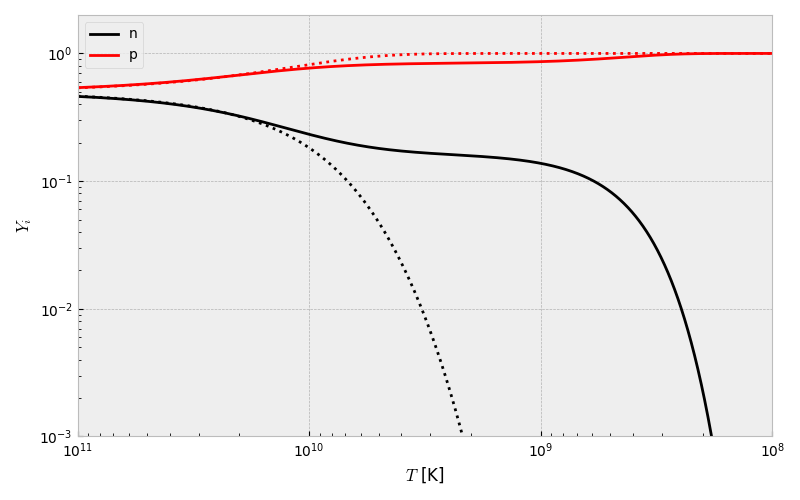
\includegraphics[width=12cm]{densities.png}
	\caption{Caption}
	\label{fig:problem_f}
\end{figure*}

\section{Problem g)}
From Problem a), we recall that
\begin{align}
	\frac{dn_i}{dt} + 3Hn_i = n_b H \frac{dY_i}{d\ln{T}}
\end{align}
Inserting
\begin{align}
	\frac{dn_i}{dt} + 3Hn_i
	\ \	=\ \ &\sum\limits_{j\neq i} [n_j\Gamma_{j\rightarrow i} - n_i\Gamma_{i\rightarrow j}] \\
		+ &\sum\limits_{jkl} [n_k n_l\gamma_{kl\rightarrow ij} - n_i n_j\gamma_{ij\rightarrow kl}]
\end{align}
and defining $\Gamma_{ij\rightarrow kl} = n_b \gamma_{ij\rightarrow kl}$, we see
that
\begin{align}
		  \frac{dY_i}{d\ln{T}}
		= \frac{1}{H}\bigg\{
		  &\sum\limits_{j\neq i} [\frac{n_j}{n_b}\Gamma_{j\rightarrow i} - \frac{n_i}{n_b}\Gamma_{i\rightarrow j}] \\
		+ &\sum\limits_{jkl} [\frac{n_k}{n_b}\frac{n_l}{n_b} n_b\gamma_{kl\rightarrow ij}
													- \frac{n_i}{n_b}\frac{n_j}{n_b} n_b\gamma_{ij\rightarrow kl}]
			\bigg\} \\
		= \frac{1}{H}\bigg\{
		  &\sum\limits_{j\neq i} [Y_j \Gamma_{j\rightarrow i} - Y_i \Gamma_{i\rightarrow j}] \\
		+ &\sum\limits_{jkl} [Y_k Y_l \Gamma_{kl\rightarrow ij}
													- Y_i Y_j \Gamma_{ij\rightarrow kl}]
			\bigg\}
\end{align}
\section{Problem h)}

\begin{acknowledgments}  % if you disagree with the spelling, blame Americans
I would like thank myself for writing this beautiful document.
\end{acknowledgments}


%% When it comes to the bibliography I personally generate it using BibLaTeX. (see the link above if you're interested)
%% You're obviously allowed to create the references section however you like.
%% I'll keep it simple here.
\section*{References}  % the asterisk (*) after \section makes the section numbering go away
\begin{itemize}
\item[-]Reference 1
\item[-]Reference 2
\end{itemize}

\newpage
%% if you want to include an appendix, this is how you do it
\appendix
\section{Name of appendix}
This will be the body of the appendix.
\section{This is another appendix}\label{appendix}
Tada.
%% all \section commands following \appendix are automatically taken as appendices

%% Note that \label{appendix} command on line 115. What this does is setup a reference point for LaTeX that you can
%% access wherever you want using \ref{appendix}.
%% You can place labels on most environments such as equations, figures, tables, etc.


%% If you want to include figure:
%\includegraphics[scale=1.0]{filename}
%% check https://en.wikibooks.org/wiki/LaTeX/Importing_Graphics if you want to know more

\end{document}
